% 原书 p.273–p.281（PDF p.281–p.289）；第 9 章 9.7 节（颈部拉伸）
% 说明：本文件不含 \chapter（第 9 章标题由 ch09a 写出）；9.7 节起于 PDF p.281 中部。
% >>> p281
\section{颈部拉伸（Neck-Stretching）}

\begin{keytakeaways}
\begin{itemize}
  \item 几何图像：沿辛流形内部的接触型超曲面 $M$ 把流形「拉长颈部」，得到一族与 $X$
        微分同胚的形变辛流形 $(X_k,\omega_k,J_k)$；令 $k\to+\infty$ 即得极限流形
        $X_\infty$，其中含多份辛化 $\R\times M$。
  \item 数学工具：Liouville 向量场与接触形式（$\iota_Y\omega=\lambda$，$\omega|_M=\dd\lambda$）、
        辛化、恰当辛配边；SFT 紧性把 $J_k$-全纯曲线列的极限解释为\textbf{全纯
        building}，其各层之间由闭 Reeb 轨道相接。
  \item 本节结论（定理 9.7.2，Cieliebak–Mohnke）：不存在恰当的拉格朗日嵌入
        $\T^n\hookrightarrow(\CP^n,\omega_{\mathrm{FS}})$。
  \item 应用要点：证明用颈部拉伸 + 定点点约束（由 Gromov–Witten 不变量保证曲线存在）
        + 面积估计，最终得到面积 $\leqslant\pi/2$ 的圆盘，与恰当性 (9.42) 要求的
        $m\pi$ 矛盾。
\end{itemize}
\end{keytakeaways}

回忆 7.3 节开头：嵌入的拉格朗日子流形 $L\overset{i}{\hookrightarrow}(M,\omega=\dd\lambda)$
（其中 $i$ 是包含映射）诱导一个上同调类，称为 \textbf{Liouville 类}
$[\lambda_L]\in H^1(L;\R)$。确切地说，$\lambda_L=i^*\lambda$，它是 $L$ 上的闭
$1$-形式。若 $i^*\lambda=\dd f$ 是恰当 $1$-形式，则称这样的 $L$ 为
$(M,\omega=\dd\lambda)$ 中的\textbf{恰当拉格朗日子流形}（exact Lagrangian
submanifold）。在 $(\R^4,\omega_{\mathrm{std}}=\dd\lambda_{\mathrm{std}})$ 中
（其中 $\lambda_{\mathrm{std}}=x_1\dd y_1+x_2\dd y_2$），有大量恰当拉格朗日子流形，
例如
\[
L=\mathrm{span}_{\R}\langle y_1,y_2\rangle=\{x_1=x_2=0\}.
\]
此时 $i^*\lambda_{\mathrm{std}}=0$，即 $f\equiv0$。然而，当限制到闭拉格朗日子流形时，
我们有如下令人惊讶的结果。

\begin{wthm}{9.7.1}（[99]）
$(\R^{2n},\omega_{\mathrm{std}}=\dd\lambda_{\mathrm{std}})$ 中不存在任何闭的、
恰当的、嵌入的拉格朗日子流形。
\end{wthm}

% [Tutor Note: 含糊点拨——定理 9.7.1 是 Gromov 1985 年非压缩性工作的推论，通常用
% 「用全纯圆盘填满」的论证证明：若存在闭恰当拉格朗日 $L$，则可数穿过 $L$ 上点的
% 全纯圆盘，其面积由恰当性控制，再用 Gromov 紧性得到矛盾。本书省略此证明（见下一段），
% 而定理 9.7.2 是它在 $\CP^n$ 中的类比；两者都体现「恰当性 ⇒ 面积约束」这一核心机制。
% 注意此处「闭」不可省：$\R^{2n}$ 中恰当地嵌入的（非闭）拉格朗日平面大量存在。]

固定嵌入拉格朗日子流形 $L\subset(M,\dd\lambda)$ 的拓扑类型，比如 $L=\T^n$（拓扑
$n$-环面），则 Liouville 类为 $[\varphi^*\lambda]\in H^1(\T^n;\R)\cong\R^n$。特别地，
对 $(\R^4,\omega_{\mathrm{std}}=\dd\lambda_{\mathrm{std}})$ 中的定向拉格朗日子流形，
Gromov 的上述结果可以重述为：不存在任何恰当嵌入
$\varphi:\T^2\to(\R^4,\omega_{\mathrm{std}}=\dd\lambda_{\mathrm{std}})$（因为由命题
1.6.1 之后那段的拓扑约束以及 [166] 的主要结果，$(\R^4,\omega_{\mathrm{std}})$ 中
仅有的闭嵌入定向拉格朗日子流形在拓扑上都是环面）。

% >>> p282
定理 9.7.1 的证明超出本书范围。本节我们将证明如下类似结果，它是 K. Cieliebak 与
K. Mohnke 的一个一般结果的特例。

\begin{wthm}{9.7.2}（[53] 中的定理 1.21）
不存在任何恰当的拉格朗日嵌入 $\T^n\hookrightarrow(\CP^n,\omega_{\mathrm{FS}})$。
\end{wthm}

这里 $(\CP^n,\omega_{\mathrm{FS}})$ 不是恰当辛流形，因此需要一个新的定义来说明嵌入
$\varphi$ 何时是恰当的。在 $\CP^n$ 中考虑标准直线 $\CP^1$，在 $\omega_{\mathrm{FS}}$
下其面积等于 $\pi$。于是称嵌入 $\varphi:\T^n\hookrightarrow(\CP^n,\omega_{\mathrm{FS}})$
为\textbf{恰当的}，如果任意嵌入圆盘
$(\mathbb D^2,\partial\mathbb D^2)\xrightarrow{f}(\CP^n,\varphi(\T^n))$ 都满足
\begin{equation}\tag{9.42}
(f^*\omega_{\mathrm{FS}})(\mathbb D^2)=m\pi,\qquad\text{对某个 }m\in\Z.
\end{equation}

% [Tutor Note: 原文疑误——原文此处把 $f$ 写成「任意嵌入圆盘」，但严格地说应要求 $f$
% 是「嵌入到 $\CP^n$ 中且边界落在 $\varphi(\T^n)$ 上」的圆盘；且 (9.42) 对\textbf{所有}
% 这样的圆盘成立，而非仅对某个 $f$。译文按原意译出，注意 (9.42) 左侧是 $f^*\omega_{\mathrm{FS}}$
% 在 $\mathbb D^2$ 上的积分（即圆盘面积），右侧要求它是 $\pi$ 的整数倍。]

\begin{wrem}{9.7.1}
若 $f$ 是 $J$-全纯圆盘，则由命题 1.4.1 的结论可知 $m>0$（当 $f$ 非平凡时）。另注意：
在 $n=1$ 的情形（此时背景流形是 $(\CP^1,\omega_{\mathrm{FS}})$），标准的「赤道」
$S^1\hookrightarrow(\CP^1,\omega_{\mathrm{FS}})$ \emph{不是}恰当的，因为上半球面
作为嵌入圆盘
$(\mathbb D^2,\partial\mathbb D^2=S^1)\xrightarrow{f}
(\CP^1=S^2,\varphi(S^1))$，其面积只有 $\CP^1$ 中标准直线（即 $\CP^1$ 自身）面积的
一半。
\end{wrem}

% [Tutor Note: 易错预警——注 9.7.1 的「一半」正是 $n=1$ 时恰当性失效的关键：
% 上半球面面积 $=\pi/2$，而 (9.42) 要求面积 $=m\pi$，无整数 $m$ 可满足。
% 这也说明「恰当性」是一个很强的面积量子化条件，而非仅仅「面积有限」。]

我们将借证明定理 9.7.2 之机，引入一个强有力的方法，称为\textbf{颈部拉伸}
（neck-stretching）。它是一个几何过程：从一条已有的 $J$-全纯曲线出发，产生一列
伪全纯曲线。这列曲线最终会「收敛」到由若干伪全纯曲线组成的（形式）组合，称为
\textbf{全纯 building}（holomorphic building）。就应用而言，人们常用此极限（或极限中
的子曲线）的信息来导出障碍或矛盾。

首先，让我们建立此过程的输入。设 $(X^{2n},\omega)$ 是带边或不带边的辛流形。设
$M^{2n-1}\subset X^{2n}$ 是\textbf{接触型}超曲面，即 $\omega|_M=\dd\lambda$ 且
$\lambda$ 是 $M$ 的接触形式。当 $(X,\omega)$ 是带边辛流形时，$M\subset X$ 可以取为
$X$ 的边界。利用 $M$ 上的这个接触形式 $\lambda$，背景流形 $X$ 可以分解为两个闭子集
之并
\[
X=\widetilde X^+\cup\widetilde X^-,
\]
使得 $\widetilde X^+\cap\widetilde X^-=M$。哪个分支标为 $\widetilde X^+$、哪个标为
$\widetilde X^-$，取决于由方程 $\iota_Y\omega=\lambda$ 在 $M$ 附近唯一确定的诱导向量
场（\textbf{Liouville 向量场}）$Y$ 的方向（cf.\ 例 3.2.3）。我们将用下面的例子来说明
这一约定。

\begin{wexam}{9.7.1}
(i) 若 $(M,\xi=\ker\alpha)$ 是切触流形，而 $X=SM=\R\times M$ 是 $M$ 的辛化，其辛
结构为 $\omega=\dd(\ee^r\alpha)$（见定义 3.2.1）。则（Liouville）向量场
$Y=\partial_r$，它指向 $\R=\R(r)$ 的正方向。
% >>> p283
因此
\[
\widetilde X^+=[0,\infty)\times M,\qquad
\widetilde X^-=(-\infty,0]\times M.
\]
关于此分解，见图 9.20。
\end{wexam}

\begin{figure}[htbp]
  \centering
  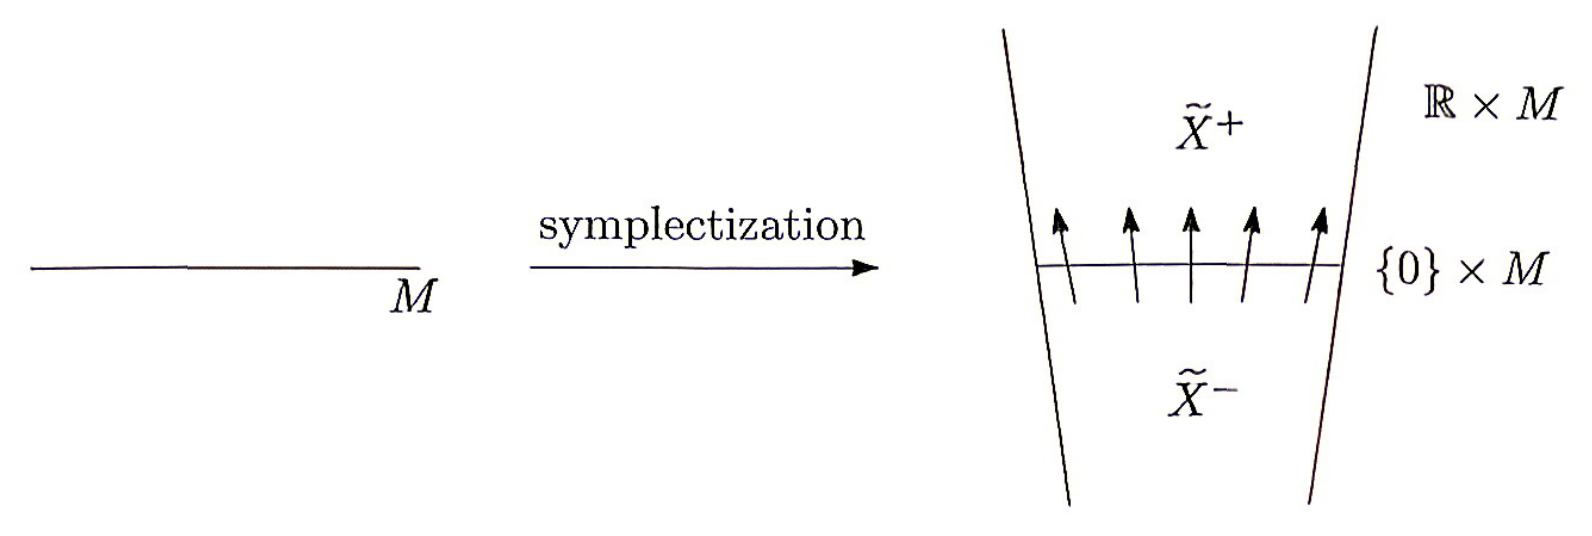
\includegraphics[width=0.9\linewidth]{figures/fig_p283_1.png}
  \caption*{图 9.20\quad 把 $M$ 的辛化分成两部分（原书 p.275, Figure 9.20；
  PDF p.283）}
\end{figure}

更具体地，我们有如下例子。

(ii) 取带黎曼度量 $g$ 的黎曼流形 $(Q,g)$。令 $X=T^*Q$，其标准辛结构为
$\omega_{\mathrm{can}}=\dd\lambda_{\mathrm{can}}$（见例 1.2.2）。取例 3.2.4 中考虑的
单位余球面丛 $M=S^*_gQ=\{(q,p)\mid\|p\|_{g^*}=1\}=\partial D^*_g(Q)$。我们知道
$\omega|_{S^*_g(Q)}=\dd\lambda_{\mathrm{can}}$。特别地，（Liouville）向量场算得为
$Y=p\partial_p$，它指向外（远离 $T^*Q$ 的零截面）。因此
\[
\widetilde X^+=\left\{(q,p)\in T^*Q\ \middle|\ \|p\|_{g^*}\geqslant1\right\},
\qquad
\widetilde X^-=\left\{(q,p)\in T^*Q\ \middle|\ \|p\|_{g^*}\leqslant1\right\},
\]
其中 $\widetilde X^+\cup\widetilde X^-=T^*Q=X$。\hfill$//$

% [Tutor Note: 易错预警——例 9.7.1 (ii) 中 $Y=p\partial_p$ 与 $\|p\|_{g^*}$ 的指标
% 容易混淆：$p$ 是余切向量，$\|\cdot\|_{g^*}$ 是余切丛上的对偶范数；$\partial_p$ 沿
% 纤维方向，故 $Y$ 指向「$p$ 增大」的方向，恰是离开零截面的方向，因此正分支是
% $\|p\|\geqslant1$。另注意 $S^*_gQ=\partial D^*_g(Q)$ 是余球面丛与余圆盘丛边界的
% 等同，这是后文把 $L$ 的管状邻域写成 $D^*_gL$ 的基础。]

下面的例子展示了人们自然遇到接触型超曲面的另一种情形。

\begin{wexam}{9.7.2}
考虑两个 Liouville 区域 $(U,\dd\lambda)$ 与 $(V,\dd\lambda)$ 之间的\textbf{恰当
辛嵌入} $\varphi:(U,\dd\lambda)\to(V,\dd\lambda)$，即满足 $\varphi^*\lambda=\lambda$
的嵌入（为简单起见，我们假设 $U$ 与 $V$ 上的原函数相同）。或者，也可以从 Liouville
区域 $(U,\dd\lambda)$ 的完备化（记作 $(\widehat W,\dd\lambda)$）出发，然后取两个
Liouville 区域 $U,V\subset\widehat W$，其辛结构分别由 $\dd\lambda$ 在 $U$ 与 $V$
上的限制给出。

容易验证 $\varphi$ 的像的边界，即 $\partial(\varphi(U))$，是 $V$ 中的接触型超平面，
其切触结构由 $1$-形式 $\lambda|_{\partial(\varphi(U))}$ 给出。（Liouville）向量场
就是由 $V$ 的定义性 Liouville 向量场给出的那个。特别地，取 $X=V$、
$M=\partial(\varphi(U))$，我们有
\[
\widetilde X^+=V\setminus\varphi(U),\qquad\widetilde X^-=\varphi(U).
\]
关于此分解，见图 9.21 左图。注意正分支
$\widetilde X^+=V\setminus\varphi(U)$ 是恰当辛流形，其辛结构就是
% >>> p284
从 $V$ 限制而来的 $\omega=\dd\lambda$。它的边界有两个连通分支：「正」边界分支
（Liouville 向量场指向外）是 $\partial V$；「负」边界分支（Liouville 向量场指向内）
是 $\partial\varphi(U)$。见图 9.21 右图。这样的几何结构称为从 $\partial\varphi(U)$ 到
$\partial V$ 的\textbf{恰当辛配边}（exact symplectic cobordism）。
\end{wexam}

\begin{figure}[htbp]
  \centering
  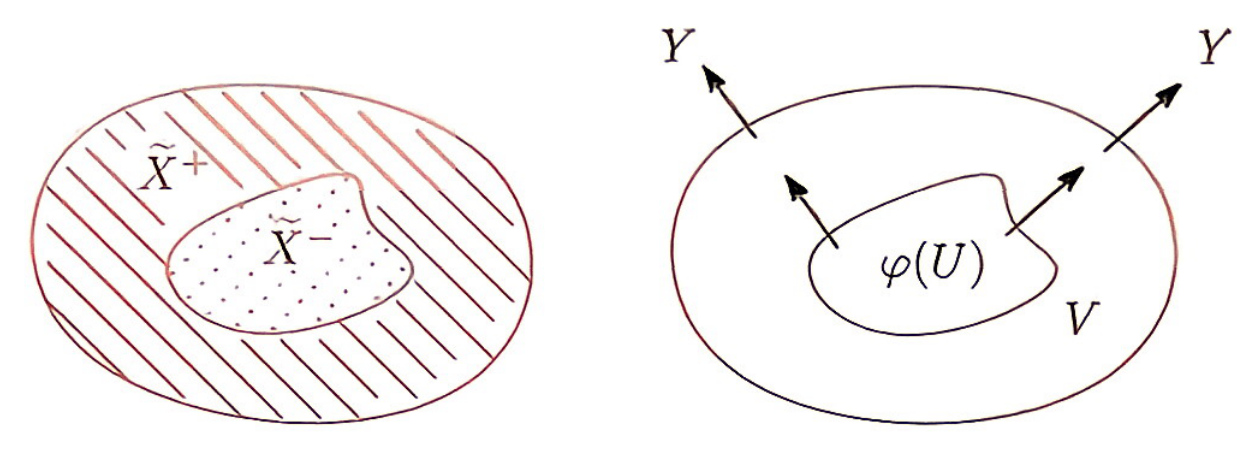
\includegraphics[width=0.72\linewidth]{figures/fig_p284_1.png}
  \caption*{图 9.21\quad 一个恰当辛配边（原书 p.276, Figure 9.21；PDF p.284）}
\end{figure}

下面的例子结合了例 9.7.1 中的 (ii) 与例 9.7.2。

\begin{wexam}{9.7.3}
设 $\psi:L\to(X,\omega)$ 是拉格朗日嵌入（于是 $\psi(L)\subset X$ 是 $(X,\omega)$
中的拉格朗日子流形）。由 Weinstein 邻域定理（定理 4.3.3），$\psi(L)\subset X$ 的
一个邻域可以辛同胚地等同于单位余圆盘丛 $D^*_gL$（对 $L$ 上某个度量 $g$）。换言之，
$(D^*_gL,\dd\lambda_{\mathrm{can}})\hookrightarrow(X,\omega)$ 是辛嵌入，且满足
$\varphi|_{0_L}=\psi$（见图 9.22）。此外，$\varphi(S^*_gL)=\partial\varphi(D^*_gL)$
是 $(X,\omega)$ 中的接触型超曲面。我们有分解
\[
X=\widetilde X^+\cup\widetilde X^-
=(X\setminus\varphi(D^*_gL))\cup\varphi(D^*_gL).
\]
若 $\partial X$ 连通且非空（且 $\partial X$ 也是接触型的），则
$\widetilde X^+=X\setminus\varphi(D^*_gL)$ 是从 $\varphi(S^*_gL)$ 到 $\partial X$ 的
恰当辛配边。\hfill$//$
\end{wexam}

\begin{figure}[htbp]
  \centering
  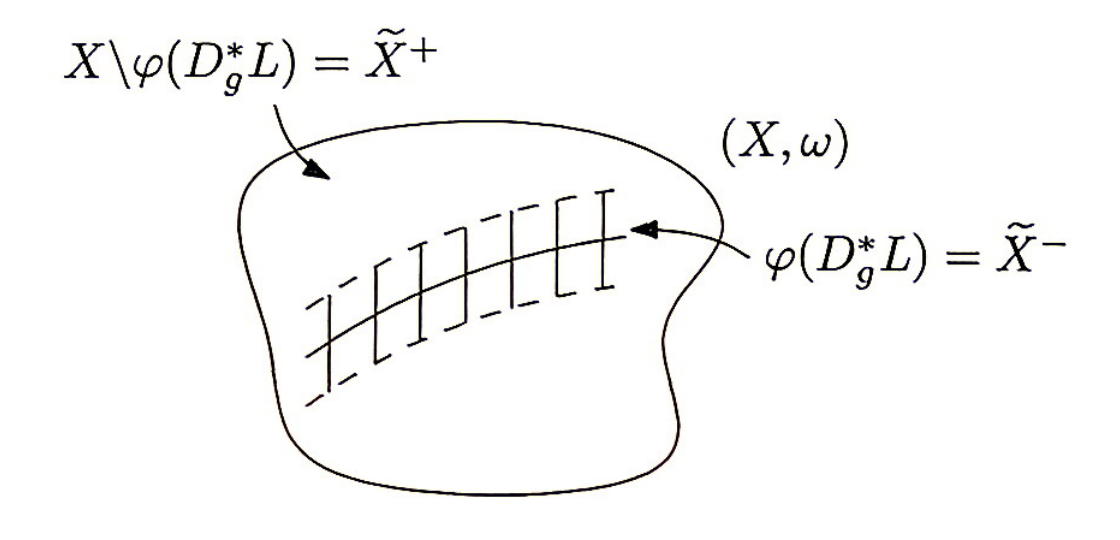
\includegraphics[width=0.62\linewidth]{figures/fig_p284_2.png}
  \caption*{图 9.22\quad 从 $\varphi(S^*_gL)$ 出发的一个恰当辛配边（原书 p.276,
  Figure 9.22；PDF p.284）}
\end{figure}

% [Tutor Note: 含糊点拨——例 9.7.3 是本节全部应用的技术核心：拉格朗日嵌入的 Weinstein
% 管状邻域把「沿 $L$ 的接触型超曲面」标准化为余球面丛 $S^*_gL$。这样颈部拉伸的
% 超曲面 $M=\varphi(S^*_gL)$ 就有了显式的模型，其上的 Reeb 流对应 $L$ 上的测地流
% （见证明定理 9.7.2 时 (i) 的论证：闭 Reeb 轨道 ↔ 闭测地线）。]

\begin{wrem}{9.7.2}
对例 9.7.3 中的嵌入 $L\to(X,\omega)$，当 $L=\T^n$ 时，对充分小的 $\varepsilon>0$
与合适的 $S>0$，可以把一个非常薄的椭球 $E(\varepsilon,S)$ 辛嵌入 $D^*_g\T^n$。因此
我们有三个层次 $E(\varepsilon,S)\hookrightarrow D^*_g\T^n\hookrightarrow X$，
% >>> p285
它们由两个恰当辛配边连接：
\[
X=\left(X\setminus\varphi(D^*_g\T^n)\right)
\cup\left(\varphi(D^*_g\T^n)\setminus\varphi(\psi(E(\varepsilon,S)))\right)
\cup\varphi(\psi(E(\varepsilon,S))).
\]
关于这种多层配边结构的应用，见 [113-114]。
\end{wrem}

给定如上输入，即一个辛流形 $(X,\omega)$ 连同其内部一个接触型超曲面 $M$（以及 $M$ 上
由 $\lambda$ 给出的接触 $1$-形式），对每个固定的 $k\in\N$，我们可以如下定义一个与
$X$ 微分同胚的辛流形
\[
X_k:=\widetilde X^+\cup_M[-k,0]\times M\cup_M\widetilde X^-,
\]
并赋予辛形式
\begin{equation}\tag{9.43}
\omega_k:=
\begin{cases}
\omega, & \text{在}\ \widetilde X^+\ \text{上},\\
\dd(\ee^r\lambda), & \text{在}\ [-k,0]\times M\ \text{上},\\
\ee^{-k}\omega, & \text{在}\ \widetilde X^-\ \text{上}.
\end{cases}
\end{equation}
然后考虑 $(X_k,\omega_k)$ 上几乎复结构 $J_k$，简单地由下式给出
\begin{equation}\tag{9.44}
J_k:=
\begin{cases}
J, & \text{在}\ \widetilde X^\pm\ \text{上}\ (J\ \text{与}\ \omega\ \text{相容}),\\
J_M, & \text{在}\ [-k,0]\times M\ \text{上},
\end{cases}
\end{equation}
其中 $J_M$ 是辛化 $(\R\times M,\dd(\ee^r\lambda))$ 上的几乎复结构，如 3.3 节开头
所指定。\textbf{颈部拉伸}就是令 $k\to+\infty$ 的过程，从而
\begin{equation}\tag{9.45}
(X_k,\omega_k,J_k)\xrightarrow{k\to+\infty}
(X_\infty,\omega_\infty,J_\infty)
:=X^+\cup_M(\R\times M)\cup_MX^-,
\end{equation}
其中 $X^+:=((-\infty,0]\times M)\cup_M\widetilde X^+$，
$X^-:=\widetilde X^-\cup_M([0,\infty)\times M)$，而中间分支 $\R\times M$ 是 $M$ 的
辛化。需要强调的是：对中间分支 $\R\times M$，由于 $\R$ 可以（形式上）等同于多个
$\R$ 粘在一起，事实上极限流形中可以有多个（但有限个）$\R\times M$ 的副本。换言之，
(9.45) 中的极限流形实际上应写成
\begin{equation}\tag{9.46}
(X_\infty,\omega_\infty,J_\infty)
=X^+\cup_M(\R\times M)\cup_M\cdots\cup_M(\R\times M)\cup_MX^-.
\end{equation}
示意图见图 9.23。

\begin{figure}[htbp]
  \centering
  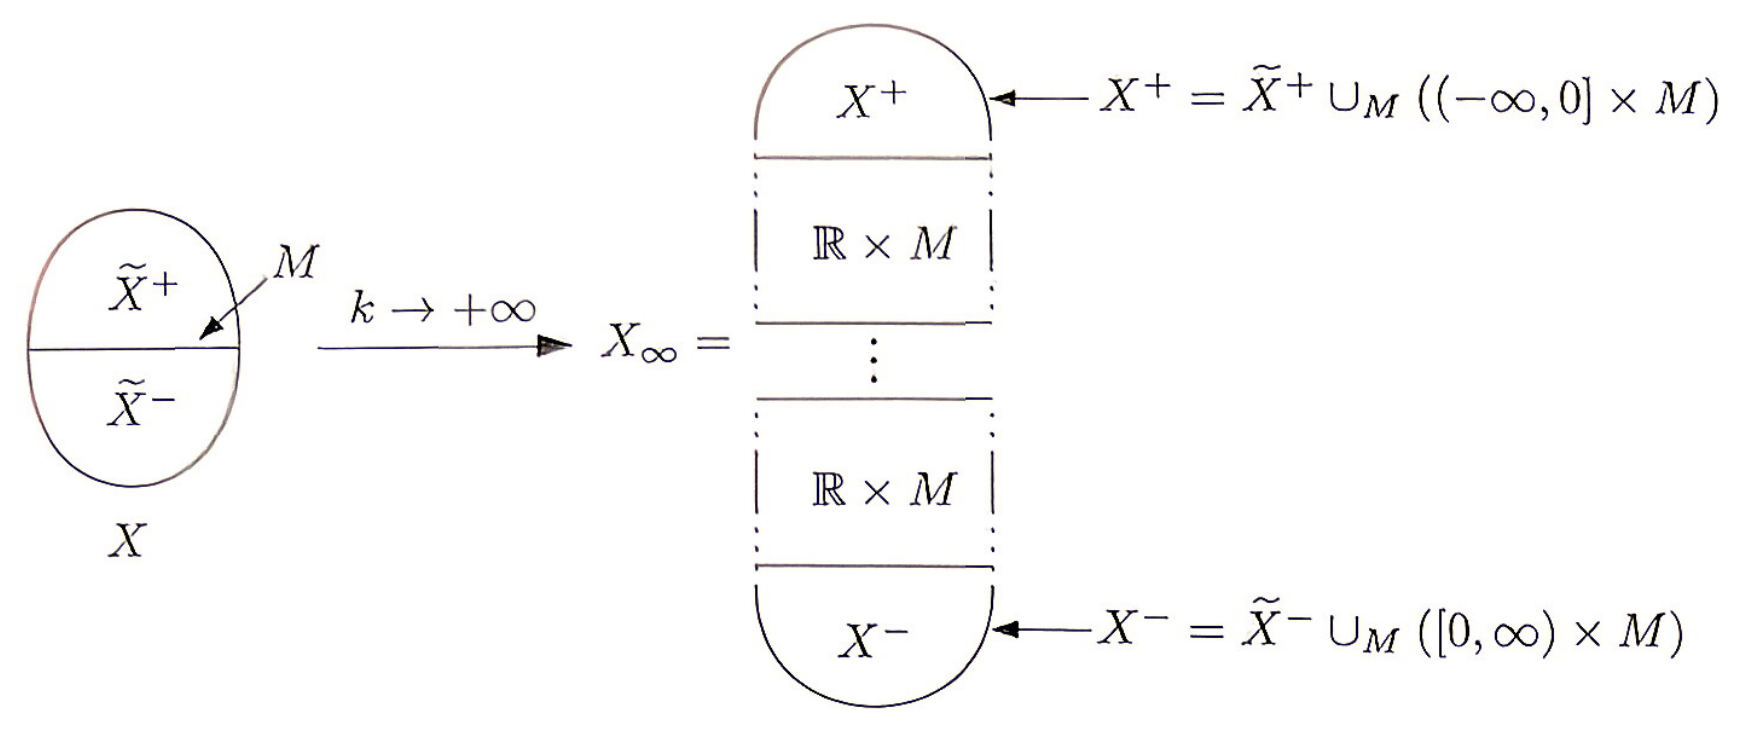
\includegraphics[width=0.95\linewidth]{figures/fig_p286_1.png}
  \caption*{图 9.23\quad 颈部拉伸过程（原书 p.278, Figure 9.23；PDF p.286）}
\end{figure}

\begin{wexam}{9.7.4}
继续例 9.7.3（考虑由拉格朗日嵌入 $\psi:L\to(X,\omega)$ 诱导的恰当辛嵌入
$\varphi:(D^*_gL,\dd\lambda_{\mathrm{can}})\to(X,\omega)$，使得
$\varphi|_{0_L}=\psi$），我们有
\[
X^+=\left((-\infty,0]\times\varphi(S^*_gL)\right)
\cup_{\varphi(S^*_gL)}\left(X\setminus\varphi(D^*_gL)\right)
=X\setminus\varphi(0_L)=X\setminus\psi(L).
\]
类似地，我们有
$X^-=\varphi(D^*_gL)\cup_{\varphi(S^*_gL)}([0,\infty)\times\varphi(S^*_gL))$。中间
分支是切触流形 $\varphi(S^*_gL)$ 的辛化，即 $S(\varphi(S^*_gL))$。
\end{wexam}

% >>> p286
可以按等价的方式把 $\varphi$ 延拓到 $[0,\infty)\times\varphi(S^*_gL)$ 上，即对任意
$r\in[0,\infty)$ 定义 $\varphi(r,x):=r\cdot\varphi(1,x)$（也就是在 $\R$-分支上作
伸缩），于是 $[0,\infty)\times\varphi(S^*_gL)=\varphi([0,\infty)\times S^*_gL)$。
因此
\begin{align*}
X^-
&=\varphi(D^*_gL)\cup_{\varphi(S^*_gL)}
\left([0,\infty)\times\varphi(S^*_gL)\right)\\
&=\varphi(D^*_gL)\cup_{\varphi(S^*_gL)}
\varphi([0,\infty)\times S^*_gL)=\varphi(T^*L).
\end{align*}
用同样的方式（但把上述延拓做到整个 $r\in\R$），我们有辛化
\[
S(\varphi(S^*_gL))=\R\times\varphi(S^*_gL)
=\varphi(\R\times S^*_gL)=\varphi(T^*L\setminus0_L).
\]
\hfill$//$

\begin{wrem}{9.7.3}
当 $(X,\omega)$ 具有切触边界时，为定义极限流形
$(X_\infty,\omega_\infty,J_\infty)$，我们总先考虑完备化 $\widehat X$（见例 3.2.3），
无论 $M$ 是否取为切触边界本身。考虑完备化的理由是：后文处理曲线时，分析要么在闭
辛流形中进行，要么在完备的（非紧）辛流形中进行。
\end{wrem}

给定辛流形 $(X,\omega)$ 及其内部一个接触型超曲面 $M$，考虑一列 $J$-全纯曲线：
\[
f_k:(\Sigma_g,j_{\mathrm{std}})\to(X_k,\omega_k,J_k),
\qquad k\in\N,
\]
其中 $(X_k,\omega_k,J_k)$ 是上面颈部拉伸过程中得到的各形变辛流形及其相容几乎复结构。
事实上，在拓扑上 $X_k$ 总是与原来的 $X$ 本身微分同胚，差别仅来自接触超曲面 $M$ 附近
的形变。与定理 8.3.2 类似——后者基于 8.3 节开头所示的「冒泡」现象——$J_k$-全纯曲线
列 $\{f_k\}_{k\in\N}$ 将收敛到一个极限
\[
f_\infty:(\Sigma_g,j_{\mathrm{std}})\to(X_\infty,\omega_\infty,J_\infty),
\]
% >>> p287
条件是同调类 $[f_k(\Sigma_g)]$ 在 $X_k(\cong X)$ 中固定、且 $f_k$ 的 $\omega_k$-能量
一致有界。此外，极限 $f_\infty(\Sigma_g)$ 一般由 (9.46) 中各层的若干分支组成：从
$X^-$ 开始，经过可能的多层 $\R\times M$，最后到 $X^+$。这一紧性结果的精确表述需要
额外的数学记号，故为简洁起见，我们用图 9.24 来说明这样的极限。重要的是，由定理
3.3.1，由于全纯曲线中每个分支的能量有界，这些曲线的渐近端是 $M$ 上的闭 Reeb 轨道。

\begin{figure}[htbp]
  \centering
  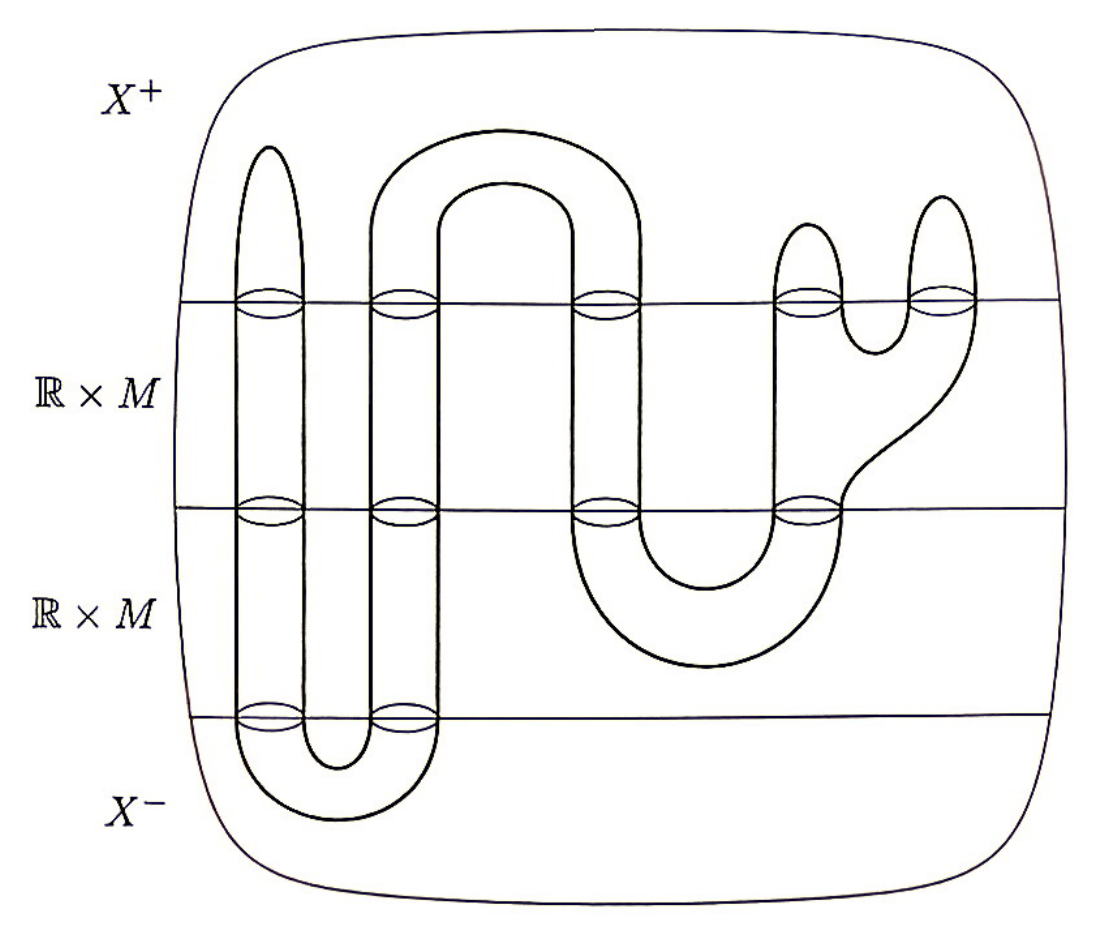
\includegraphics[width=0.62\linewidth]{figures/fig_p287_1.png}
  \caption*{图 9.24\quad 极限流形 $(X_\infty,\omega_\infty,J_\infty)$ 中的极限曲线
  （原书 p.279, Figure 9.24；PDF p.287）}
\end{figure}

这样的极限称为\textbf{全纯 building}。它从 $f_k$ 继承了许多数据。例如，亏格 $g$ 在
极限中保持不变；$f_k$ 的能量收敛到一个数（所得全纯 building 的能量），它可以通过
把 building 中各分支的能量相加来计算；指标之间也有类似的关系（由闭情形中的
$c_1(TX)$ 与渐近闭 Reeb 轨道的 Conley–Zehnder 指标共同度量）。特别地，对带边辛流形
$(X,\omega)$（例如 $V\setminus\varphi(U)$），这些数据的创造性组合通常被用来获得
配边 $V\setminus\varphi(U)$ 存在性的障碍。这最终导致辛嵌入 $\varphi:U\to V$ 的障碍
（见 [113-114]）。关于紧性结果的更详细阐述，见 [53] 中的定理 2.9 以及 C. Abbas 的
专著 [1]。

% [Tutor Note: 含糊点拨——这里的紧性就是 SFT（辛场论）紧性定理（Bourgeois–Eliashberg–
% Hofer–Wysocki–Zehnder）：在能量一致有界与同调类固定的条件下，$J_k$-全纯曲线列
% 收敛为全纯 building，而 building 的「层与层之间」由 $M$ 上的闭 Reeb 轨道连接。
% 本书把它作为黑箱引用（[53] 定理 2.9 与 [1]），但读者应记住三条要点：
% (1) 能量有界是本质条件；(2) 极限中各分支的亏格之和、能量之和、指标之和分别守恒；
% (3) 每个分支的渐近端都是闭 Reeb 轨道。这三条正是后面定理 9.7.2 证明的全部输入。]

要对如上描述的伪全纯曲线应用颈部拉伸技术，还需要确认：对每个 $J_k$，确实存在
$J_k$-全纯曲线 $f_k$（换言之，可挑选的伪全纯曲线应当足够多）。然而这往往是最困难的
部分，因为我们需要对一族几乎复结构（而非单个几乎复结构）确认曲线的存在性。

% >>> p288
对闭辛流形，Gromov–Witten 不变量（8.5 节研究过）常常可以帮忙。

\begin{wexam}{9.7.5}
在 $\CP^n$ 上回忆：当 $i+j+k=2n+1$ 时
$\mathrm{GW}^{\CP^n}_{L,3}(c^i,c^j,c^k)=1$（见事实 8.7.1），其余情形为零。于是
固定 $i=n$（这样 $c^n$ 对应于 $\CP^n$ 中的一个点），再要求 $J$-全纯曲线经过
$\CP^n$ 中的另一个点（它占据另一个 $c^n$），由这一计算可知这样的曲线仍然存在。
而且，这对颈部拉伸过程中构造的 (9.44) 中每个形变几乎复结构 $J_k$ 都成立，因为
Gromov–Witten 不变量与其构造中相容几乎复结构的选择无关。这个「经过另一个点」的条件
可以从流形层面推广到切空间层面，称为\textbf{相切条件}（tangency condition，见 [53]
的 3.2 节）。\hfill$//$
\end{wexam}

% [Tutor Note: 易错预警——例 9.7.5 的要点是「Gromov–Witten 不变量与 $J$ 无关」这一
% 事实：它保证在颈部拉伸得到的整族 $J_k$ 上都有曲线存在，否则无法取极限。注意
% $\mathrm{GW}^{\CP^n}_{L,3}(c^i,c^j,c^k)$ 中 $c$ 是上同调类、$L$ 是直线类；三个插入
% 的度数条件 $i+j+k=2n+1$ 是维数匹配的结果（本书采用的分次约定见 8 章）。]

正如所承诺的，我们将给出定理 9.7.2 的证明；这个证明是演示如何应用颈部拉伸技术的
绝佳例子。

\begin{wproof}[定理 9.7.2 的证明]
我们将用反证法证明。假设存在恰当的拉格朗日嵌入
$\psi:\T^n\to(\CP^n,\omega_{\mathrm{FS}})$。在 $\T^n$ 上固定一个度量 $g$，使得每条
闭测地线都非可缩。由例 9.7.3，在对度量 $g$ 作伸缩后，存在辛嵌入
$\varphi:D^*_g\T^n\to(\CP^n,\omega_{\mathrm{FS}})$，使得
$\varphi|_{0_{\T^n}}=\psi$。特别地，像 $\varphi(S^*_g\T^n)$ 是
$(\CP^n,\omega_{\mathrm{FS}})$ 中的接触型超曲面。

我们将沿超曲面 $\varphi(S^*_g\T^n)$ 实施颈部拉伸过程。考虑一列 $J_k$-全纯球面
$f_k:(S^2,j_{\mathrm{std}})\to(\CP^n,\omega_k,J_k)$，其中 $\omega_k$ 与 $J_k$ 分别是
(9.43) 中的形变辛结构与 (9.44) 中的形变几乎复结构。加上拓扑约束：同调类
$[f_k(S^2)]\in H_2(\CP^n;\Z)$ 表示标准直线类，记作 $L$。于是容易验证
\[
f_k\ \text{的}\ \omega_k\text{-面积}
=\int_{S^2}f_k^*\omega_k\leqslant[\omega_{\mathrm{FS}}](L)=\pi.
\]
固定 $D^*_g\T^n$ 中一点 $p$，并加上「点点约束」：对每个 $k\in\N$，像 $f_k(S^2)$
还必须经过 $p$。由于 $(\CP^n,\omega_{\mathrm{FS}})$ 中伪全纯曲线的丰富性（见例
9.7.5），我们不会损失上面选取的曲线列 $\{f_k\}_{k\in\N}$ 中的任何曲线。现在由紧性，
$f_k$ 收敛到极限曲线
$f_\infty:(S^2,j_{\mathrm{std}})\to(\CP^n,\omega_\infty,J_\infty)$。这里，由定义性
分解 (9.46) 与例 9.7.4，
\[
(\CP^n,\omega_\infty,J_\infty)
=(\CP^n\setminus\psi(\T^n))
\cup_{\varphi(S^*_g\T^n)}(\R\times\varphi(S^*_g\T^n))
\cup_{\varphi(S^*_g\T^n)}\cdots
\cup_{\varphi(S^*_g\T^n)}\varphi(T^*\T^n).
\]
特别地，$X^+=\CP^n\setminus\psi(\T^n)$，且 $X^-=\varphi(T^*\T^n)$（在如例 9.7.4
那样把 $\varphi$ 等价延拓到 $T^*\T^n$ 之后）。对所得的全纯 building
$f_\infty(S^2)$，我们有如下观察。
\begin{enumerate}[label=(\roman*)]
  \item $X^-=\varphi(T^*\T^n)$ 中每个分支至少有两个正端（见图 9.25）。事实上，由
        我们对 $g$ 的选取，$S^*_g\T^n$ 上的任意闭 Reeb 轨道——它对应于
        % >>> p289
        $(\T^n,g)$ 中的一条闭测地线——都是非可缩的。一个正端（$X^-$ 中某分支的）
        若只有单个，就意味着其渐近轨道可缩、并被一个圆盘盖住。
\end{enumerate}
\end{wproof}

\begin{figure}[htbp]
  \centering
  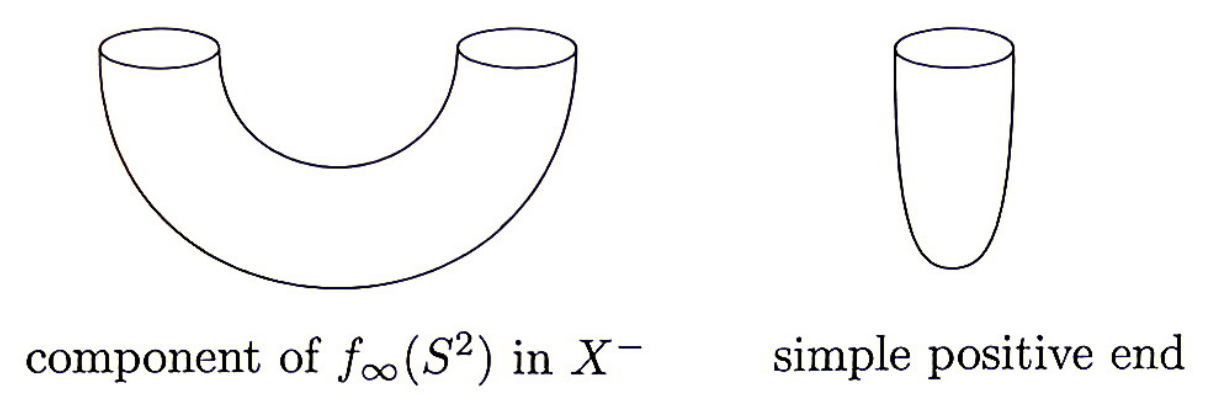
\includegraphics[width=0.78\linewidth]{figures/fig_p289_1.png}
  \caption*{图 9.25\quad $X^-$ 中每个分支至少有两个正端（原书 p.281,
  Figure 9.25；PDF p.289）}
\end{figure}

\begin{wproof}[定理 9.7.2 的证明（续）]
\begin{enumerate}[label=(\roman*),start=2]
  \item $X^+=\CP^n\setminus\psi(\T^n)$ 中必须至少有两个分支（见图 9.26 左图）。
        全纯 building $f_\infty(S^2)$ 的亏格（即把 $f_\infty(S^2)$ 内部所有分支沿其
        渐近端粘起来所得拓扑曲面的亏格）等于零，即 $S^2$ 的亏格。由上面的 (i)，
        若 $X^+=\CP^n\setminus\psi(\T^n)$ 中只有一个分支，就会迫使这个全纯 building
        出现洞（hole）。示意图见图 9.26 右图。
  \item 由上面 (ii) 的一个初等论证，$X^+=\CP^n\setminus\psi(\T^n)$ 中至少有一个
        分支是拓扑圆盘 $D$。更明确地说，这是 $\CP^n$ 中一个边界落在 $\psi(\T^n)$ 内的
        伪全纯圆盘。然而，再次由 (ii)，这个圆盘 $D$ 的 $\omega_\infty$-面积至多为
        $\omega_\infty(f_\infty(S^2))/2\leqslant\pi/2$。最后，由于 $D$ 位于 $X^+$
        内，而在 $X^+$ 中所有形变辛结构 $\omega_k$ 都保持为 $\widetilde X^+$ 上的
        $\omega_{\mathrm{FS}}$（$\omega_\infty$ 亦然），$D$ 的 $\omega_\infty$-面积
        实际上等于 $D$ 的 $\omega_{\mathrm{FS}}$-面积，从而不超过 $\pi/2$。这与
        $\psi$ 的恰当性定义 (9.42) 矛盾。于是我们得到所需的矛盾。
\end{enumerate}
\end{wproof}

\begin{figure}[htbp]
  \centering
  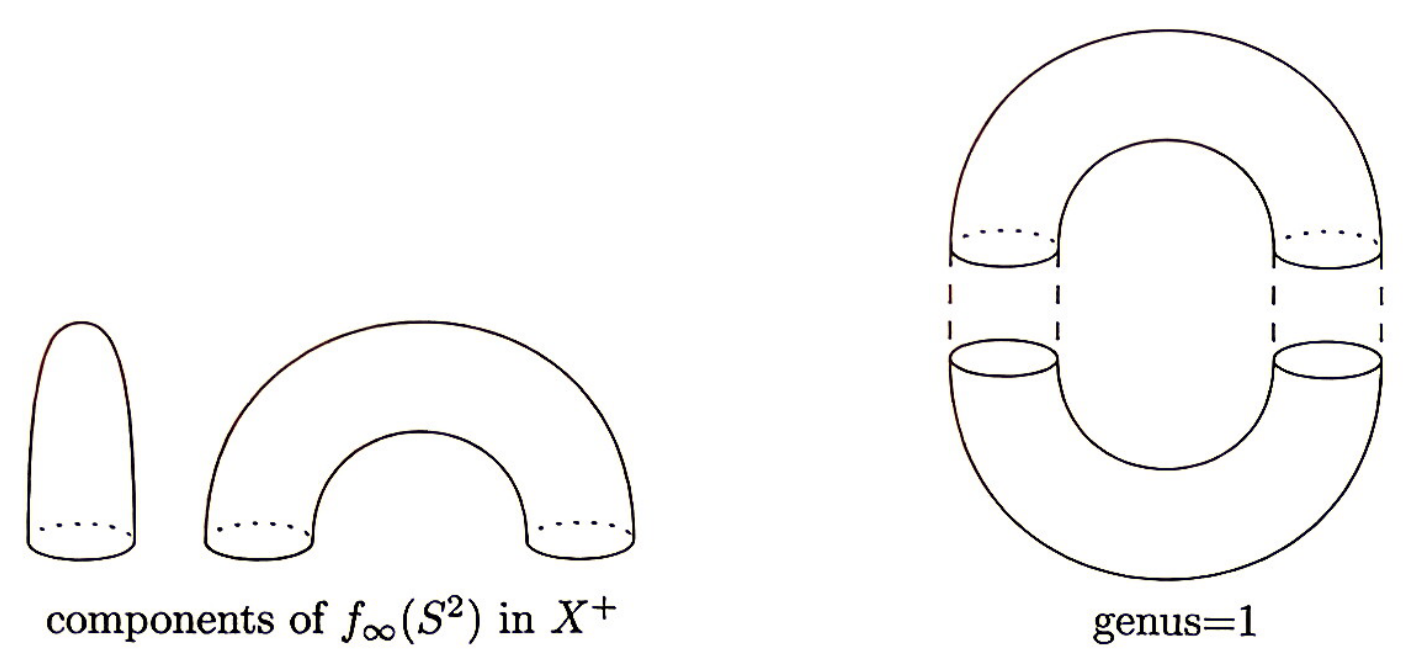
\includegraphics[width=0.8\linewidth]{figures/fig_p289_2.png}
  \caption*{图 9.26\quad $X^+$ 中至少有两个分支（原书 p.281, Figure 9.26；
  PDF p.289）}
\end{figure}

% [Tutor Note: 含糊点拨——证明的逻辑链值得逐条核对：(i) 用「非可缩测地线」保证
% 每个负侧分支至少两个正端；(ii) 由于 building 的亏格为 $0$（来自 $S^2$），正侧若
% 只有一个分支就会产生洞（亏格 ≥1），矛盾，故正侧至少两个分支；(iii) 于是至少有一个
% 正侧分支是圆盘，其面积 ≤ 总能量的一半 ≤ π/2，与 (9.42) 要求的 $m\pi$ 矛盾
% （π/2 不是 π 的整数倍）。注意三个「至少/至多」都要用到：面积上界来自总能量 π，
% 除以 2 来自「至少两个分支」，而 (9.42) 的量子化条件排除了 π/2。]

% [Tutor Note: 原文疑误（轻微）——(i) 中「A single positive end (of a component in
% $X^-$) simply means that the asymptotic orbit is contractible, capped by a disk」：
% 严格说「单个正端」意味着该分支的渐近 Reeb 轨道可缩，于是可在 $X^-$ 内用一个
% 全纯圆盘盖住（填满）；原文的 capped by a disk 是此意。译文照原文语义译出。
% 另本页「$X^-$ 中每个分支至少有两个正端」的论证依赖 Reeb 流 ↔ 测地流的对应
% （$S^*_g\T^n$ 上的 Reeb 轨道即 $\T^n$ 的闭测地线），见例 9.7.3 的 Tutor Note。]
